%% For double-blind review submission
%\documentclass[sigplan,review,anonymous]{acmart}
%% For single-blind review submission
%\documentclass[sigplan,review]{acmart}
%% For proofreading
% \documentclass[sigplan,authordraft]{acmart}
%% For final camera-ready submission
\documentclass[sigplan]{acmart}
%% For booklet
% \documentclass[acmsmall]{acmart}

% !TEX root=../main.tex


%% Basics %%%%%%%%%%%%%%%%%%%%%%%%%%%%%%%%%%%%%%%%%%%%%%%%%%%%%%%%%%%%%%%%%%%%%%

%% Fixes %%

\usepackage{underscore}


%% Fonts %%

\usepackage[utf8]{inputenc}
\usepackage[T1]{fontenc}

\usepackage{stmaryrd}

% \usepackage{tgpagella}
% \usepackage{lucidabr}
\usepackage{libertine}
\usepackage[varqu]{zi4}
\usepackage[libertine]{newtxmath}


%% Programming %%

\usepackage{ifthen}


%% Layout %%

% \usepackage[final]{microtype}


%% Additions %%%%%%%%%%%%%%%%%%%%%%%%%%%%%%%%%%%%%%%%%%%%%%%%%%%%%%%%%%%%%%%%%%%

%% Textual %%

\usepackage{paralist}
\usepackage{quoting}


%% Maths %%

\usepackage{amsmath}
\usepackage{mathpartir}


%% Graphics %%

\usepackage{graphicx}
% \usepackage{xcolor}


%% Tabulations %%

\usepackage{booktabs}
\usepackage{array}


%% Listings %%

% \usepackage[final]{listings}


%% References %%

\usepackage{cleveref}

% !TEX root=../main.tex


%% Fixes %%

\frenchspacing

%% NOTE: uses the same lengths as in `tufte-common.def` and `article.cls`...
\setlength{\bigskipamount}   {3.25ex plus .2ex} %% ...before (sub)section
\setlength{\medskipamount}   {2.3ex  plus .2ex} %% ...after section
\setlength{\smallskipamount} {1.5ex  plus .2ex} %% ...after subsection


%% Numbering %%

% \setcounter{secnumdepth}{2}


%% Compact lists %%
%% NOTE: requires `paralist`

\setlength{\pltopsep}{\smallskipamount}
\setlength{\plpartopsep}{\parskip}
\setlength{\plitemsep}{\parskip}
\setlength{\plparsep}{\parskip}

% !TEX root=../main.tex


%% Helpers %%%%%%%%%%%%%%%%%%%%%%%%%%%%%%%%%%%%%%%%%%%%%%%%%%%%%%%%%%%%%%%%%%%%%

\let\newoperator\DeclareMathOperator


%% Text %%%%%%%%%%%%%%%%%%%%%%%%%%%%%%%%%%%%%%%%%%%%%%%%%%%%%%%%%%%%%%%%%%%%%%%%

\newcommand*{\alert}[1]
  {\textbf{#1}}
\newcommand*{\enquote}[1]
  {``#1''}
\newcommand*{\todo}[1]
  {\ensuremath{\star}\marginnote{\ensuremath{\star}#1}}


%% Lists %%
%% NOTE: requires `paralist`

%% Use compact lists by default
\renewenvironment{itemize}
  {\begin{compactitem}}
  {\end{compactitem}}
\renewenvironment{enumerate}
  {\begin{compactenum}}
  {\end{compactenum}}
\renewenvironment{description}
  {\begin{compactdesc}}
  {\end{compactdesc}}
%% Define starred versions as in-paragraph-lists
\newenvironment{itemize*}
  {\begin{inparitem}}
  {\end{inparitem}}
\newenvironment{enumerate*}
  {\begin{inparenum}}
  {\end{inparenum}}
\newenvironment{description*}
  {\begin{inpardesc}}
  {\end{inpardesc}}


%% Blocks %%

\newenvironment{block}
  {\smallskip}
  {\smallskip}


%% Column types %%
%% NOTE: requires `array`

\newcolumntype{L}{>{$}l<{$}}
\newcolumntype{C}{>{$}c<{$}}
\newcolumntype{R}{>{$}r<{$}}
\newcolumntype{T}{>{\ttfamily}l}
\newcolumntype{S}{>{\sffamily}l}


%% References %%
%% NOTE: requires `cleveref`

\let\see\cref
\let\See\Cref
\let\at\cpageref


%% Citations %%
%% NOTE: requires `natbib`

\let\cite\citep
\let\textcite\citet


%% Math %%%%%%%%%%%%%%%%%%%%%%%%%%%%%%%%%%%%%%%%%%%%%%%%%%%%%%%%%%%%%%%%%%%%%%%%

%% NOTE: change this to \emptyset when using a font that includes a nice standard emptyset
\let\nothing\varnothing


%% Braces %%

\let\<\langle
\let\>\rangle

\newcommand*{\llbrace}
  {\{\!|}
\newcommand*{\rrbrace}
  {|\!\}}


%% Operators %%

\let\lt<
\let\gt>
\let\eq\equiv

\newcommand*{\pp}
  {+\!\!+}


%% Shortcuts %%

\newcommand*{\powerset}
  {\mathcal{P}}

\newcommand*{\NN}{\mathbb{N}}
\newcommand*{\ZZ}{\mathbb{Z}}
\newcommand*{\RR}{\mathbb{R}}
\newcommand*{\CC}{\mathbb{C}}

\newcommand*{\LL}{\mathbb{L}}
\newcommand*{\UU}{\mathbb{U}}
\newcommand*{\BB}{\mathbb{B}}
\renewcommand*{\SS}{\mathbb{S}}

\newoperator{\downto}
  {\;\rightarrow\!\shortmid\;}

\let\to\rightarrow
\let\implies\Rightarrow
\let\infers\vdash

% !TEX root=../main.tex


%% Styles %%%%%%%%%%%%%%%%%%%%%%%%%%%%%%%%%%%%%%%%%%%%%%%%%%%%%%%%%%%%%%%%%%%%%%

\lstdefinestyle{natural}
  {columns=fullflexible
  ,gobble=2
  ,breaklines=true
  ,breakatwhitespace=true
  ,literate=
    %{.}{{$\cdot$}}1
    %{.}{{\ }}1
    {<<}{{$\<$}}1
    {>>}{{$\>$}}1
    {->}{{$\to$\ }}2
    % {--}{{--}}1
    %{_}{{\ }}1
    %{\ "}{{\ \textquotedblleft}}2
    %{"\ }{{\textquotedblright\ }}2
  ,basicstyle={\sffamily}
  ,keywordstyle=[1]{\bfseries}
  ,keywordstyle=[2]{\scshape}
  ,keywordstyle=[3]{}
  %,commentstyle={\itshape}
  %,identifierstyle={\itshape}
  ,emphstyle={\itshape}
  %,stringstyle={\rmfamily}
  ,showstringspaces=false
  ,texcl=true
  ,mathescape=true
  %,escapechar=\$
  %,escapeinside={\{\}}
  ,xleftmargin=1\parindent
  }

\lstdefinestyle{flexible}
  {columns=flexible
  ,gobble=2
  ,fontadjust=true
  ,basicstyle={\ttfamily\small}
  ,commentstyle={\itshape}
  ,keywordstyle={\bfseries}
  %,identifierstyle={\itshape}
  %,stringstyle={\ttfamily}
  ,emphstyle={\itshape}
  ,showstringspaces=false
  ,texcl=true
  ,mathescape=true
  %,escapechar=\$
  %,escapeinside={\{\}}
  ,xleftmargin=1\parindent
  }

\lstdefinestyle{literate}
  {literate=
    {\\}{{$\lambda$}}1
    {\\\$}{{\$}}1 %NOTE: otherwise eaten by `\`, NOTE: prevents \$ to be parsed as math escape
    {\\/}{{$\vee$}}1
    {/\\}{{$\wedge$}}1
    {A.}{{$\forall$}}1
    {E.}{{$\exist$}}1
    {->}{{$\rightarrow$ }}1
    {<-}{{$\leftarrow$}}1
    {<=}{{$\leq$}}1
    {>=}{{$\geq$}}1
    {>>=}{{>>=}}3 %NOTE: otherwise eaten by `>=`
    {\{|}{{$\{\!|\!$}}1
    {|\}}{{$\!|\!\}$}}1
    {\{|*|\}}{{$\{\!|\!\!\star\!\!|\!\}$}}3
  }


%% Definitions %%%%%%%%%%%%%%%%%%%%%%%%%%%%%%%%%%%%%%%%%%%%%%%%%%%%%%%%%%%%%%%%%

%% Tasks %%

\lstdefinelanguage{tasks}
  {sensitive=true
  ,morekeywords=[1]{if,then,else,case,of}
  ,morekeywords=[2]{Bool,Int,String,Store,List}
  ,morestring=[b]"
  ,morecomment=[l]--
  ,morecomment=[n]{\{-}{-\}}
  }[keywords,strings,comments]
\lstdefinestyle{tasks}
  {style=natural
  ,literate=
    {\\}{{$\lambda$}}1
    {>>=}{{$\Then$\ }}1
    {>>?}{{$\Next$\ }}1
    {<&>}{{$\And$\ }}1
    {<|>}{{$\Or$\ }}1
    {<?>}{{$\Xor$\ }}1
    {edit}{{$\Edit$}}1
    {enter}{{$\Enter$}}1
    {store}{{$\Change$}}1
    {fail}{{$\Fail$}}1
    {==}{{$\equiv$\ }}1
    {/=}{{$\nequiv$\ }}1
  }

\lstnewenvironment{TASK}[1][]
  {\lstset{language=tasks,style=tasks,#1}}
  {}
\newmacro{TS}[1][1]
  {\lstinline[language=tasks,style=tasks,#1]}
\newmacro{includeTASK}[2][]
  {\lstinputlisting[language=tasks,style=tasks,#1]{#2}}


%% Flows %%

\lstdefinelanguage{flows}
  {sensitive=true
  ,morekeywords=[1]{module,where,define,using,as,yielding,share,holding,with,do,for,fork,then,when,next,done,on,and,or,not,readonly,writeonly,readwrite}
  ,morekeywords=[2]{Bool,Int,String,Shared,List, Date,Document,Photo, Citizen,Company,Declaration}
  ,morekeywords=[3]{True,False,Just,Nothing,List}
  ,morestring=[b]"
  ,morecomment=[l]--
  ,morecomment=[n]{\{-}{-\}}
  }[keywords,strings,comments]

% \lstMakeShortInline[language=flows,style=natural] | % |
\lstnewenvironment{FLOW}[1][]
  {\lstset{language=flows,style=natural,#1}}
  {}
\newmacro{FL}[1][1]
  {\lstinline[language=flows,style=natural,#1]}
\newmacro{includeFLOW}[2][]
  {\lstinputlisting[language=flows,style=natural,#1]{#2}}


%% Clean %%

\lstdefinelanguage{clean}
  {sensitive=true
  %,alsoletter={ABCDEFGHIJKLMNOPQRSTUVWXYZabcdefghijklmnopqrstuvwxyz_`}
  %,alsoletter={~!@\#$\%^\&*-+=?<>:|\\} %$
  ,morekeywords={from,definition,implementation,import,module,system,code,inline,if,case,of,let,let!,in,where,with,class,instance,generic,derive,dynamic,infix,infixl,infixr}
  ,morestring=[b]"
  ,morestring=[b]'
  ,morecomment=[l]//
  ,morecomment=[n]{/*}{*/}
  }[keywords,strings,comments]

\lstnewenvironment{CLEAN}[1][]
  {\lstset{language=clean,style=flexible,#1}}
  {}
\newmacro{CL}[1][1]
  {\lstinline[language=clean,style=flexible,#1]}
\newmacro{includeCLEAN}[2][1]
  {\lstinputlisting[language=clean,style=flexible,#1]{#2}}


\newlogo[ITASKS]{iTasks}
\newlogo{BPMN}
\newlogo{BPEL}
\newlogo{UML}
\newlogo{WFN}

\newlogo{EDSL}
\newlogo{GUI}

\newlogo{STW}
\newlogo{NWO}


\acmConference[PLDI'19]
  {International Conference on Programming Language Design and Implementation}
  {June 2019}
  {Phoenix, Arizona, United States}
\acmYear{2019}

%\acmISBN{978-x-xxxx-xxxx-x/YY/MM}
%\acmDOI{10.1145/nnnnnnn.nnnnnnn}

%\startPage{1}

\settopmatter{printfolios=true,printccs=false,printacmref=false}
\setcopyright{none}             %% For review submission
%\setcopyright{acmcopyright}
%\setcopyright{acmlicensed}
%\setcopyright{rightsretained}
%\copyrightyear{2017}           %% If different from \acmYear


%% Bibliography style
\bibliographystyle{ACM-Reference-Format}
%% Citation style
%\citestyle{acmauthoryear}  %% For author/year citations
\citestyle{acmnumeric}      %% For numeric citations
%\setcitestyle{nosort}      %% With 'acmnumeric', to disable automatic
                            %% sorting of references within a single citation;
                            %% e.g., \cite{Smith99,Carpenter05,Baker12}
                            %% rendered as [14,5,2] rather than [2,5,14].
%\setcitesyle{nocompress}   %% With 'acmnumeric', to disable automatic
                            %% compression of sequential references within a
                            %% single citation;
                            %% e.g., \cite{Baker12,Baker14,Baker16}
                            %% rendered as [2,3,4] rather than [2-4].



\begin{document}

%% Title information
\title{Interactive Processes: A Formal Foundation for Task-Oriented Programming}
                                        %% [Short Title] is optional;
                                        %% when present, will be used in
                                        %% header instead of Full Title.
%\titlenote{with title note}             %% \titlenote is optional;
                                        %% can be repeated if necessary;
                                        %% contents suppressed with 'anonymous'
%\subtitle{Revisited edition}            %% \subtitle is optional
%\subtitlenote{with subtitle note}       %% \subtitlenote is optional;
                                        %% can be repeated if necessary;
                                        %% contents suppressed with 'anonymous'


%% Author information
%% Contents and number of authors suppressed with 'anonymous'.
%% Each author should be introduced by \author, followed by
%% \authornote (optional), \orcid (optional), \affiliation, and
%% \email.
%% An author may have multiple affiliations and/or emails; repeat the
%% appropriate command.
%% Many elements are not rendered, but should be provided for metadata
%% extraction tools.

\author{Markus Klinik}
%\authornote{with author1 note}          %% \authornote is optional; can be repeated if necessary
%\orcid{nnnn-nnnn-nnnn-nnnn}             %% \orcid is optional
\affiliation{
  %\position{PhD}
  \department{Department of Software Science}
  %\department{Institute for Computing and Information Sciences}
                                        %% \department is recommended
  \institution{Radboud University}
                                        %% \institution is required
  \streetaddress{Toernooiveld 212}
  \postcode{6525 EC}
  \city{Nijmegen}
  %\state{State1}
  \country{The Netherlands}
}
\email{m.klinik@cs.ru.nl}               %% \email is recommended

\author{Nico Naus}
%\authornote{with author1 note}          %% \authornote is optional; can be repeated if necessary
%\orcid{nnnn-nnnn-nnnn-nnnn}             %% \orcid is optional
\affiliation{
  %\position{PhD}
  \department{Department of Software Systems}
                                        %% \department is recommended
  \institution{Utrecht University}      %% \institution is required
  \streetaddress{Princetonplein 5}
  \postcode{3584 CC}
  \city{Utrecht}
  %\state{State1}
  \country{The Netherlands}
}
\email{n.naus@uu.nl}                    %% \email is recommended

\author{Tim Steenvoorden}
%\authornote{with author1 note}          %% \authornote is optional; can be repeated if necessary
%\orcid{nnnn-nnnn-nnnn-nnnn}             %% \orcid is optional
\affiliation{
  %\position{PhD}
  \department{Department of Software Science}
  %\department{Institute for Computing and Information Sciences}
                                        %% \department is recommended
  \institution{Radboud University}      %% \institution is required
  \streetaddress{Toernooiveld 212}
  \postcode{6525 EC}
  \city{Nijmegen}
  %\state{State1}
  \country{The Netherlands}
}
\email{tim@cs.ru.nl}                     %% \email is recommended

% \author{Rinus Plasmeijer}
% %\authornote{with author2 note}       %% \authornote is optional; can be repeated if necessary
% %\orcid{nnnn-nnnn-nnnn-nnnn}             %% \orcid is optional
% \affiliation{
%   %\position{prof.}
%   % \department{Department of Software Science}
%   \department{Institute for Computing and Information Sciences}
%                                         %% \department is recommended
%   \institution{Radboud University}
%                                         %% \institution is required
%   \streetaddress{Toernooiveld 212}
%   \city{Nijmegen}
%   %\state{State1}
%   \postcode{6525 EC}
%   \country{The Netherlands}
% }
% \email{rinus@cs.ru.nl}                  %% \email is recommended


%% Paper note
%% The \thanks command may be used to create a "paper note" ---
%% similar to a title note or an author note, but not explicitly
%% associated with a particular element.  It will appear immediately
%% above the permission/copyright statement.
%\thanks{with paper note}                %% \thanks is optional
                                        %% can be repeated if necesary
                                        %% contents suppressed with 'anonymous'


%% Abstract
%% Must come before \maketitle command
\begin{abstract}
  % !TEX root=../pldi2019.tex

Task-Oriented Programming (\TOP) is a programming paradigm that focusses on modelling real world collaborations between people.
It prescribes a declarative programming style to specify multi-user workflows.
Workflows can be higher-order.
They communicate through typed values on a local or global level.
Such specifications can be turned into interactive applications for different platforms,
supporting collaboration during execution.

In this paper we decompose the rich features of \TOP into elementary language elements,
which makes them suitable for formal treatment.
We use the simply typed lambda calculus, extended with pairs and references, as a base language.
On top of this language, we develop \TOPHAT (TopHat), a calculus for modular interactive workflows.

We describe \TOPHAT by means of a layered semantics.
These layers consist of multiple big step evaluations on expressions,
and two labelled transition systems, handling user inputs.
We show some interesting properties of this machinery.
This approach allows for comparison with other work in the field.
We place \TOPHAT in perspective with the process calculus \CSP.

\end{abstract}

% \begin{teaserfigure}
%    \includegraphics[width=\textwidth]{figures/declrequest-part.pdf}
%    \caption{This is a teaser}
%    \label{fig:teaser}
% \end{teaserfigure}

%% 2012 ACM Computing Classification System (CSS) concepts
%% Generate at 'http://dl.acm.org/ccs/ccs.cfm'.

%% End of generated code


%% Keywords
%% comma separated list, optional
%\keywords{workflow, dataflow, visual programming, program generation}


%% Note: \maketitle command must come after title commands, author
%% commands, abstract environment, Computing Classification System
%% environment and commands, and keywords command.
\maketitle


% !TEX root=../main.tex



\section{Introduction}

%XXX: Alejandro:
% The introduction seems to be more about why Task-Oriented Programming is nice and useful.
% Personally, I would like it to tell me another story:
% given that some people find TOP useful (as shown by the many examples),
% why should be care about formalising it and which challenges does it pose?
% I think this is what people from ICFP would care about more.
%NOTE: Ik hoop dat de `Challenges` sectie dit wat opvangt. --TS

Many applications these days are developed to support workflows in institutions and businesses.
Take for example expense declarations, order processing, and emergency management.
Some of these workflows occur on the boundary between organisations and customers,
like flight bookings or tax returns.
What they all have in common is
that they need to interact with different people (end users, tax officers, customers, etc.)
and they use information from multiple sources (input forms, databases, sensors, etc.).

\subsection{Tasks}

We call interactive units of work based on information sources \emph{tasks}.
% Tasks stand for units of work in the real world, assigned to people.
Tasks model real world collaboration between users,
are driven by work users do,
and are assigned to some user.
Users could be people out in the field or sitting behind their desks,
as well as machines doing calculations or fetching data.



\subsection{Task-oriented programming}
\label{sec:top}

%XXX: Alejandro: Not entirely convincing
% Hij heeft het hier volgens mij over de titel van de sectie en het woord aims in de eerste zin. Misschien moeten we een hardere claim doen hier? --NN
% Ik heb `aims` vervangen door `targets`. Doet dat wat? --TS

% Task-Oriented Programming (\TOP) is a programming paradigm aimed at writing interactive multi-user applications in a declarative way \cite{conf/ppdp/PlasmeijerLMAK12}.
Task-oriented programming (\TOP) is a programming paradigm which targets the sweet spot between faithful modelling workflows
and rapid prototyping of multi-user web applications supporting these workflows \cite{conf/ppdp/PlasmeijerLMAK12}.
% Task-oriented programming (\TOP) is a programming paradigm to support these ways of working.
\TOP focusses on modelling collaboration patterns.
This gives rise to a user's need to interact and share information.
Next to that, \TOP automatically provides solutions to common development jobs like designing \GUI{s}, connecting to databases, and communicating between servers and clients.

Therefore,
a language that supports \TOP should choose the right level of abstraction to support two things.
% \TOP has two aspects.
% First, it should allow to specify tasks from real world scenarios.
Firstly, it should provide primitive building blocks that are useful for high-level descriptions of how users collaborate,
with each other and with machines.
These building blocks are: \emph{editors}, \emph{composition}, and \emph{shared data}.
% Second, it should be able to generate multi-user web applications to support these scenarios.
Secondly, it should be able to generate applications, including graphical user interfaces, from workflows modelled with said building blocks.

Users can work together in a number of ways, and this is reflected in \TOP by task compositions.
There is \emph{sequential} composition, \emph{parallel} composition, and \emph{choice}.
Users need to communicate in order to engage in these forms of collaboration.
This is reflected in \TOP by three kinds of communication mechanisms.
There is data flow \emph{alongside} control flow, where the result of a task is passed onto the next.
There is data flow \emph{across} control flow, where information is shared between multiple tasks.
Finally, there is communication with the \emph{outside} world, where information is entered into the system via input events.
The end points where the outside world interacts with \TOP applications are called editors.
In generated applications, editors can take many forms, like input fields, selection boxes, or map widgets.



\subsection{Utilisation}


Currently, we know of two frameworks implementing \TOP: \ITASKS and \MTASKS.

\ITASKS is an implementation of \TOP, in the form of a shallowly embedded domain-specific language in the lazy functional programming language Clean.
It is a library that provides editors, monadic combinators, and shared data sources.
\ITASKS uses the generic programming facilities of Clean to derive rich client and server applications from a single source.
It has been used to model an incident management tool for the Dutch coast guard~\cite{conf/iscram/LijnseJP12}.
Also it has been used numerous times to prototype ideas for Command and Control~\cite{theses/nlda/Kool17, theses/radboud/Stutterheim17}, and in a case study for the Dutch tax authority~\cite{conf/sfp/StutterheimAP17}.

\MTASKS is a subset of \ITASKS,
focussing on \IOT devices and deployment on micro controllers.
It has been used to control home thermostats and other home automation applications \cite{koopman2018task}.
%
Both implementations currently lack formal semantics which are suited to prove properties about tasks.



\subsection{Challenges}

% \ITASKS is the de-facto reference implementation of \TOP.
Both \ITASKS and \MTASKS have been designed for developing real-world applications.
They are constantly being extended and improved with this goal in mind.
The different variations of task combinators and the details that come with real-world requirements,
make it hard to see what the essence of \TOP is.
% One of the defining aspects of both \ITASKS and \MTASKS is their embedding in a functional programming language.
% This creates a synergy where they profit from the expressivity of Clean, while enhancing the language with functionality for user interaction.
Also, the tight integration of both frameworks with Clean, makes it difficult to see where the boundaries are.
This makes formal reasoning about \TOP programs impossible.

In this paper, we want to take a step back and look at the spirit of \TOP.
We do this both formally and informally.
Informally in the sense that we give an intuitive description of the features that define task-oriented programming.
Formally in the sense that we develop a calculus which formalises these features as language constructs,
and we give them a semantics in the style that is common in programming language research.
We separate the task layer and the underlying host language, both syntactically and semantically.
Thus making explicit which properties of \TOP come from the task layer, and which come from functional programming.
Our challenge, therefore, is to model the properties of \TOP into a calculus
and pave the way for formal treatment of \TOP programs.
We give this formal calculus the name \TOPHAT (TopHat).



\subsection{Contributions}

Our contributions to workflow modelling, functional programming language design, and rapid application development are as follows.


\begin{itemize}
  \item
    We describe the essential concepts of task-oriented programming.

  \item
    We present a formal calculus for modelling declarative workflows, embedded in a simply typed lambda-calculus, called \TOPHAT.
    It is based on the aforementioned essential \TOP concepts.

  \item
    We develop a layered operational semantics for \TOPHAT that is driven by user input.
    The semantics of the task language is clearly separated from the semantics of the underlying host language.

  \item
    Along with this semantics, we present the following semantic observations on tasks:
    the current value, whether a term is stuck, the current user interface, and the accepted inputs.

  \item
    We prove progress and type preservation for \TOPHAT.

  \item
    Using both the essential concepts and the formal calculus, we compare \TOP with related work in areas ranging from business process modelling, to process algebras and reactive programming.

  \item
    We implemented the whole semantic system in the dependently typed programming language Idris \cite{journals/jfp/Brady13}.

  \item
    To create executable applications, we implemented the task layer of \TOPHAT in iTasks.
    This also demonstrates that the former is a subset of the latter.


\end{itemize}


\subsection{Structure}

In \cref{sec:example} we demonstrate the functionality of \TOPHAT by means of an example,
\Cref{sec:intuition} gives an overview of the essential concepts of \TOP.
\Cref{sec:language} introduces the \TOPHAT calculus syntax
and \cref{sec:semantics} the semantics.
Then in \cref{sec:properties} we show that certain properties hold for the calculus.
We take a look at related work in \cref{sec:relatedwork}
and conclude in \cref{sec:conclusions}.

% !TEX root=../pldi2019.tex

\section{Example}

\lstset{emph={p, ps, ss}}

In this section we develop a small example program to demonstrate the capabilities of \TOPHAT.
The example is a simple flight booking system.
It demonstrates communication with the environment, communication between parallel tasks, synchronisation, and input validation.

The application works as follows.
\begin{enumerate*}
  \item A user has to input a list of passengers for which to book tickets.
  \item At least one of these passengers has to be an adult.
  \item After a valid list of passengers has been input, the user has to pick seats.
  \item Only free seats may be picked.
  \item Every passenger must have exactly one seat.
  \item Multiple users should be able to book tickets at the same time.
\end{enumerate*}
For this example we assume that the host language has lists and two functions on them: intersect and difference.
For brevity, we omit the type annotations of variable bindings.

We start by defining some type aliases.
A passenger is a pair with name and age.
A seat is a pair with a row number and a seat letter.
A booking contains a list of passengers and a list of seats.
\begin{TASK}
  type Passenger = String * Int
  type Seat = Int * String
\end{TASK}

Choosing seats requires reading and updating shared information.
The list of free seats is stored in a reference called \TS{freeSeats}.
\begin{TASK}
  let freeSeats = ref [<<1,"A">>, <<1,"B">>, <<1,"C">>, ...] in
\end{TASK}

The flight booking task starts with entering a valid list of passengers,
denoted by \TS{enter (List Passenger)}.
A passenger is valid if the name is not empty and the age is at least 0.
A list of passengers is valid if each passenger is valid, and at least one of the passengers is an adult.
When the user has entered a valid list of passengers, the step after \TS{>>?} becomes enabled,
and the user can proceed to picking seats.
\begin{TASK}
  let valid = \p. not (fst p == "") /\ snd p >= 0 in
  let adult = \p. snd p >= 18 in
  let allValid = \ps. all valid ps /\ any adult ps in
  let bookFlight = enter (List Passenger) >>? \ps.
    if allValid ps then chooseSeats ps else fail in
\end{TASK}
A selection of seats is correct if every entered seat is free.
\begin{TASK}
  let correct = \ss. intersect ss !freeSeats == ss in
  let chooseSeats = \ps. enter (List Seat) >>? \ss.
    if correct ss /\ length ps == length ss
      then confirmBooking ps ss else fail in
\end{TASK}
The function \TS{confirmBooking} removes the picked seats from the shared list of free seats,
and displays the end result using the \TS{edit}-construct.
\begin{TASK}
  let confirmBooking = \ps. \ss.
    freeSeats := difference !freeSeats ss; edit <<ps, ss>> in
\end{TASK}
% It uses a function \TS{difference}, which removes all elements from the second list from the first list.

The main task appoints the \TS{bookFlight} task to three different users: \TS{u1}, \TS{u2}, and \TS{u3},
and run these tasks in parallel.
%%NOTE: parentheses make the line to long...
\begin{TASK}
  u1 @ bookFlight <&> u2 @ bookFlight <&> u3 @ bookFlight
\end{TASK}

\begin{figure}[h]
  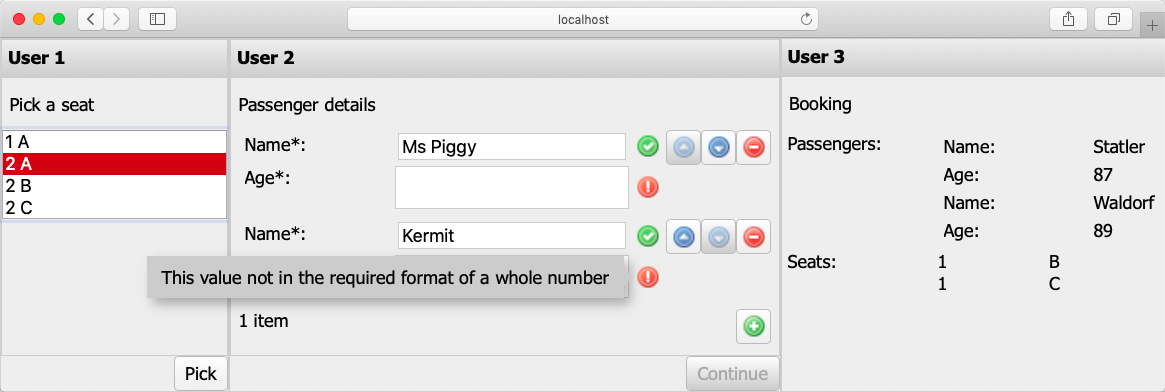
\includegraphics[width=\columnwidth]{figures/flight-booking.png}
  \caption{
    Running web application of the flight booking example using a translation to \ITASKS,
    a \TOP implementation.
    It shows three users booking a flight simultaneously.
    The first user entered name and age and continued to picking seats.
    The second is entering details of two passengers.
    The ages are not filled in, and therefore the \TS{Continue} button is disabled.
    The third user finished a booking.
    Note the first user can't pick seats \smallcaps{1b} and \smallcaps{1c} any more.
    Also, the message bubble shows it is only allowed to enter an integer in the \TS{age} field.
  }
  \label{fig:flight-booking}
\end{figure}

% !TEX root=../icfp2019.tex



\section{Related work}
\label{sec:relatedwork}

\fixme{Intro related work}


\subsection{Task-oriented programming implementations}

\paragraph{iTasks}

As mentioned earlier, iTasks is an implementation of \TOP. iTasks has many
features, and its basic combinators are versatile and powerful. Simpler
combinators are implemented by restricting the powerful ones. This is useful for
everyday programming, where having lots of functionality at one's fingertips is
convenient and efficient.

There have been two previous papers that describe semantics of iTasks, by
\citet{conf/ifl/KoopmanPA08} and \citet{conf/ppdp/PlasmeijerLMAK12}.
Both give a different semantics in the form of minimal implementations of a
subset of the interface of iTasks. These semantics however do not make an
explicit distinction between the host language and task language and they do not
provide a formal semantics, which makes formal reasoning difficult.

\paragraph{mTasks}
\fixme{Hier iets gezelligs over mTasks}
% Our work differs in three major ways.
% First, we make an explicit distinction between the host language and the task
% language, to emphasise their boundaries.
% Second, we make use of separate semantic functions for querying the current task
% value, determining the continuation after an input event, and producing a user
% interface.
% In iTasks and its aforementioned semantics, these are integrated into the
% \CL{Task} datatype.
% Third, our system does not have the notion of task stability.
% When desired, stability can be introduced by the programmer, but the system
% itself makes no use of it.
% We argue that this does not impact the expressiveness of our language.

% mTasks is another implementation of TOP, designed for coordination of IoT devices. \alert{cite MSc Lubbers}
% mTasks has been used in a demonstrator for home automation. \alert{cite MSc Andrade}



\subsection{Worfklow modelling}

Much research has been done into workflow modelling. These works focus on
describing the collaboration between subsystems, rather than the communication
between them.
The systems described here follow a \emph{boxes and arrows} model of specifying workflows.
Control flow, represented by arrows, usually can go unrestricted from anywhere to anywhere else in a workflow.
We see \TOP as the functional programming of workflows, as opposed to this \emph{goto}-style.


\paragraph{Workflow patterns}

Workflow patterns are regarded as special kind of the design patterns in
software engineering. They identify recurring patterns in workflow systems, much
like the combinators defined by \TOPHAT. Work by \citet{journals/dpd/AalstHKB03}
defines a comprehensive list of these
pattens, and examines their availability in industry workflow software.
Workflow patterns are usually described in terms of control flow graphs, and no
formal specification is given, which makes comparison and formal reasoning more
difficult.

\paragraph{Workflow Nets}

Workflow Nets~(\WFN)\cite{journals/jcsc/Aalst98} allow for the modelling and analysis
of business processes. They are graphical in nature, and clearly display how
every component is related to each other. A downside of \WFN is that
they do not facilitate higher order constructs and that they are often not
directly executable.

\paragraph{YAWL}

This is not always the case however. A language based on \WFN that is
actually directly executable is \YAWL by \citet{DBLP:journals/is/AalstH05}.
It facilitates modelling and execution of
dynamic workflows, with support for \emph{and}, \emph{or} and \emph{xor} workflow patterns. As
mentioned, \YAWL programs consist of \WFN, and are therefore programmed
visually.

\paragraph{BPEL}

\BPEL~\cite{bpel} is another popular business process language. The standardised
language allows for the specification of actions within business processes,
using an \XML format. Processes specified in \BPEL are executable, just like \YAWL.

\fixme{Is this higher order? What combinators can be used? Other limitations?}


\subsection{Process algebras}

There are two main differences between \TOP and process algebras.
The first is a difference in scope.
Process algebras focus on modelling the input/output behaviour of processes, by explicitly stating which actions are sent and received at certain points in the program.
The goal of process algebras is formal reasoning about the interaction between processes.
Typically, one wishes to prove properties such as deadlock-freedom, liveness, or adherence to a protocol specification.

The focus of \TOP on the other hand is to model collaboration patterns, with the explicit goal of not having to specify how exactly subtasks communicate.
The declarative specification of data dependencies between subtasks enables \TOP to hide such details.

The second difference concerns internal communication.
There are two forms of communication between tasks: Passing values to continuations and sharing data.
This is different from communication in process algebras, which is based on message-passing.


\paragraph{Similarities}
There are some aspects that are similar in \TOPHAT and process algebras.
Internal communication in Hoare's CSP \cite{books/Hoare85CSP} is introduced with the concealment operator.
The semantics of CSP requires that all concealed actions are handled to exhaustion before any action with the environment can take place.
This is somewhat similar to \TOPHAT, where all enabled internal steps must be taken until the system can react to input events again.
Contrast this with Milner's CCS \cite{books/Milner89CAC}, where concealed actions are visible to the outside as $\tau$-actions, and can be interleaved with external communication.

Another similarity between \TOPHAT and process algebras, or any system with concurrency for that matter, is the need for synchronisation.
Broadly speaking, concurrency means that different parts of a program can interact with the environment independently, in an interleaved manner.
Synchronisation means that only some, but not all, of the possible interleavings are desirable.
The semantics of the step combinators in \TOPHAT, together with the fact that internal communication happens atomically, allows for concise TODO: say that synchronisation in TOPHAT is the best.


\subsection{Reactive programming}

\paragraph{Esterel \& HipHop}

\paragraph{Functional reactive programming}

Functional Reactive Programming (\FRP) is a paradigm to describe dynamic changes of values in a declarative way.
This is done by specifying networks of values, called behaviours, that can depend on each other and on external events.
Behaviours can change over time, or triggered by events.
When a behaviour changes, all other behaviours that depend on it are updated automatically.
The underlying implementation that takes care of the updating usually can tie input devices, like mouse and keyboard, to event streams and behaviours to output facilities, like text fields.
This allows for declarative specifications of applications with user interfaces.

The idea of \FRP was pioneered by \citet{conf/icfp/ElliottH97}.
In the meantime there are many variants and implementations, where reactive-banana \cite{reactive-banana}, FrTime \cite{CooperK04}, and Flapjax \cite{conf/oopsla/MeyerovichGBCGBK09} belong to the most well-known.

\FRP and \TOP are different systems that have different goals in mind.
Whereas \FRP expresses automatically updating data dependencies, \TOP expresses collaboration patterns.
\TOP has no notion of time.
Tasks can not change spontaneous over time, while behaviours can.
Only input events can change task values.
The biggest conceptual difference between a workflow in \TOP and a data network in \FRP is that an event to a task only causes updates up until the next step, while an event in \FRP propagates through the whole network.

That being said, there are some concepts that are similar in \TOP and \FRP.
The \emph{stepper} behaviour, for example, is associated with an event and yields the value of the most recent event.
This is similar to editors in \TOP.
Furthermore, both systems can be used to declaratively program user interfaces, albeit in \FRP the programmer has to construct the \GUI elements manually, and connect inputs and outputs to the correct events and behaviours.
In \TOP graphical user interfaces are automatically derived.


\subsection{Session types}

Session types are a type discipline that can be used to check whether communicating programs conform to a certain protocol.
Session types are expressions in some process calculus that describe the input/output behaviour of such programs.
Session types are useful for programming languages where modules communicate with each other via messages, like \CSP, \PICALC, or Go, to name a few.
The only form of messages in \TOP are input events which drive execution, but modules do not communicate using messages.
Therefore, session types are not applicable to \TOP in the sense used in the literature.

Formal reasoning about \TOP programs is one of our future goals for \TOPHAT.
The ideas and techniques of session types could be useful for specifying that a list of inputs of a certain form leads to desired task values.
The details are a topic for future work.


\subsection{Related web services}


\paragraph{IFTTT}

If This Then That (\IFTTT)~\cite{IFTTT} is a web service that allows users to write and
configure simple conditional statements called applets, that can interact with
web services and IoT devices. These applets can be seen as tiny workflows, that
facilitate collaboration between different services and platforms. The
complexity of the flow is very limited however, and is not geared towards humans
collaborating.

\paragraph{Google forms \& Wufoo}

Google Forms~\cite{googleforms} and SurveyMonkey~\cite{wufoo} (and their various other tools like Wufoo, Precise Polling and Zoomerang) are web based survey administration apps that allows
users to compose forms and gather data from them. They are comparable to \TOP and
iTasks in that they provide an easy way for users to construct forms on the web.
However, Google Forms and Wufoo do not allow users to define what the system
then should do with this information, and can therefore not be regarded as a
workflow or business process modelling systems.

\paragraph{Chorus} % (http://www.chorus-home.org/)

Chorus~\cite{chen2017chorus} is a visual programming environment for online
collaboration apps. The goal of Chorus is to allow users to program their own
application, though which a collective task can be coordinated. Users work on a
preset data-type that drives the behaviour of the user defined applications.

% !TEX root=../pldi2019.tex

\section{Conclusion}

\paragraph{Future work}



%% Acknowledgments
\begin{acks}                            %% acks environment is optional
                                        %% contents suppressed with 'anonymous'
  %% Commands \grantsponsor{<sponsorID>}{<name>}{<url>} and
  %% \grantnum[<url>]{<sponsorID>}{<number>} should be used to
  %% acknowledge financial support and will be used by metadata
  %% extraction tools.
  % \footnotesize
  % !TEX root=../icfp2019.tex

The authors are grateful to Johan Jeuring, Sjaak Smetsers, and Andreas Vinter-Hviid for fruitful discussions,
and Rinus Plasmeijer, Peter Achten and Pieter Koopman for proofreading.

This research is supported by the Dutch Technology Foundation STW, which is part
of the Netherlands Organisation for Scientific Research (NWO), and which is
partly funded by the Ministry of Economic Affairs.

\end{acks}


%% Bibliography
\bibliography{bibliography}


%% Appendix
% \appendix
% \section{Appendix}

%Text of appendix \ldots

\end{document}
